\documentclass[12pt]{article}
\usepackage[T1]{fontenc}
\usepackage[T1]{polski}
\usepackage[utf8]{inputenc}
\newcommand{\BibTeX}{{\sc Bib}\TeX}
\usepackage{graphicx}
\usepackage{amsfonts}
\usepackage{amsmath}
\usepackage{listings}

\setlength{\textheight}{21cm}

\lstset{basicstyle=\ttfamily\footnotesize, columns=fullflexible, frame=lines,
        numbers=left, numberstyle=\tiny, showstringspaces=false, breaklines=true}

\title{{\bf Zadanie nr 1 - Trening neuronu liniowego regułą delta z~użyciem wielu wzorców treningowych}\linebreak
Inteligentna Analiza Danych}
\author{Jędrzej Małaczyński 264351 \and Jędrzej Kostyk 264339}
\date{25 października 2026}

\begin{document}
\clearpage\maketitle
\thispagestyle{empty}
\newpage
\setcounter{page}{1}
\section{Cel zadania}

Celem zadania było zaimplementowanie treningu pojedynczego neuronu liniowego
regułą delta dla zbioru złożonego z~wielu wzorców treningowych oraz zbadanie,
jak przebieg i~wynik treningu zależą od relacji między liczbą wag neuronu $N$
a~liczbą wzorców $M$. Dla każdego z~przypadków $N<M$, $N=M$ i~$N>M$ sprawdzono,
czy wagi końcowe zależą od wag początkowych oraz czy możliwe jest bezbłędne
nauczenie neuronu całego zbioru treningowego. Obserwacje zinterpretowano,
traktując trening jako rozwiązywanie układu $M$ równań liniowych z~$N$ niewiadomymi.

\section{Wstęp teoretyczny}

Neuron liniowy o~wektorze wag $\mathbf{w}\in\mathbb{R}^N$ odpowiada na wzorzec
$\mathbf{x}^{\mu}$ wartością $y^{\mu}=\mathbf{w}^{T}\mathbf{x}^{\mu}$. Trening
polega na takim doborze wag, aby odpowiedzi były jak najbliższe wartościom
żądanym $z^{\mu}$, tj.~na minimalizacji błędu średniokwadratowego (MSE)
na zbiorze treningowym~\cite{wyklad1,haykin2009}.
Zastosowano regułę delta (Widrowa--Hoffa, LMS)~\cite{widrow1960} w~wariancie
\textit{on-line} odpowiadającym Algorytmowi~3.2 z~wykładu~\cite{wyklad1}:
w~każdej epoce wzorce są prezentowane kolejno, a~wagi są poprawiane po każdym z~nich
\begin{equation}
 \mathbf{w} \leftarrow \mathbf{w} + \eta\,(z^{\mu}-\mathbf{w}^{T}\mathbf{x}^{\mu})\,\mathbf{x}^{\mu},
 \qquad \mu = 1,\dots,M .
 \label{eq_delta}
\end{equation}
Po zebraniu wzorców w~wiersze macierzy $X\in\mathbb{R}^{M\times N}$, a~wartości
żądanych w~wektor $\mathbf{z}\in\mathbb{R}^{M}$, bezbłędny trening oznacza
rozwiązanie układu $X\mathbf{w}=\mathbf{z}$. Zgodnie z~twierdzeniem
Kroneckera--Capellego dla danych losowych (rząd $X$ pełny z~prawdopodobieństwem~1)
układ jest: dla $N<M$ -- na ogół sprzeczny, dla $N=M$ -- oznaczony, a~dla $N>M$
-- nieoznaczony (rozwiązania tworzą podprzestrzeń afiniczną wymiaru $N-M$)~\cite{osowski2000}.
Jako wynik odniesienia użyto $X^{+}\mathbf{z}$, gdzie $X^{+}$ jest pseudoodwrotnością
Moore'a--Penrose'a~\cite{penrose1955}: dla $N<M$ jest to rozwiązanie
najmniejszych kwadratów (LS), dla $N=M$ -- $X^{-1}\mathbf{z}$, a~dla $N>M$
-- rozwiązanie o~minimalnej normie.

Kluczowa własność reguły~(\ref{eq_delta}): każda poprawka jest wielokrotnością
wektora wzorca $\mathbf{x}^{\mu}$, więc leży w~przestrzeni rozpiętej przez wzorce.
Składowa wag początkowych $\mathbf{w}_0$ leżąca w~jądrze $\ker X$ (prostopadła
do wszystkich wzorców) nigdy nie jest zmieniana. Jeśli układ jest niesprzeczny
i~algorytm zbiega, to wagi końcowe powinny mieć postać
\begin{equation}
 \hat{\mathbf{w}} = X^{+}\mathbf{z} + (I - X^{+}X)\,\mathbf{w}_0 ,
 \label{eq_pred}
\end{equation}
gdzie $(I - X^{+}X)$ jest rzutem ortogonalnym na $\ker X$. Hipotezę tę zweryfikowano
eksperymentalnie.

\section{Eksperymenty i wyniki}

Wspólne założenia wszystkich eksperymentów:
\begin{itemize}
 \item składowe wzorców i~wartości żądane losowane z~rozkładu $U(-1,1)$ przy stałym
       ziarnie generatora (42) -- \textbf{ten sam zbiór treningowy} we wszystkich wykonaniach,
 \item wagi początkowe z~$U(-1,1)$, \textbf{inne w~każdym wykonaniu} (ziarna 100--104),
 \item współczynnik uczenia $\eta = 0{,}01$, liczba epok $K = 10\,000$, 5~wykonań na przypadek,
 \item po każdej epoce liczono MSE na całym zbiorze treningowym; po treningu
       -- maksymalny błąd bezwzględny $\max_{\mu}|z^{\mu}-y^{\mu}|$ oraz odległości
       euklidesowe między wagami,
 \item implementacja w~Pythonie (NumPy), $X^{+}$ liczone funkcją \texttt{pinv} z~modułu \texttt{numpy.linalg}.
\end{itemize}

%%%%%%%%%%%%%%%%%%%%%%%%%%%%%%%%%%%%%%%%%%%%%%%%%%%%%%%%%%%%%%%%%%%%%%%%%%%%%%%%%%%%%%%%%%%%%%%%%%%%%%%%%%%%%%%%%
% PODROZDZIAŁ PT. EKSPERYMENT NR 1
%%%%%%%%%%%%%%%%%%%%%%%%%%%%%%%%%%%%%%%%%%%%%%%%%%%%%%%%%%%%%%%%%%%%%%%%%%%%%%%%%%%%%%%%%%%%%%%%%%%%%%%%%%%%%%%%%

\subsection{Eksperyment nr 1 -- mniej wag niż wzorców ($N=2$, $M=6$)}

\subsubsection{Założenia}

Neuron o~$N=2$ wagach trenowano na $M=6$ wzorcach, co odpowiada układowi
6~równań z~2~niewiadomymi. Macierz $X$ ma rząd~2 i~współczynnik uwarunkowania
$\mathrm{cond}(X)=1{,}21$, więc rozwiązanie LS jest jednoznaczne.

\subsubsection{Przebieg}

Algorytm uruchomiono 5~razy z~różnych wag początkowych. Wagi końcowe porównano
między sobą oraz z~rozwiązaniem LS $X^{+}\mathbf{z}$. Dodatkowo, aby wyjaśnić
niewielką różnicę między wynikiem reguły delta a~rozwiązaniem LS, powtórzono
trening dla różnych wartości $\eta$ ($K = 100\,000$ epok).

\subsubsection{Rezultat}

Wyniki przedstawiono w~Tab.~\ref{tab_n2m6}, a~przebieg błędu na Rys.~\ref{fig_n2m6}.
\begin{table}[h!]
 \caption{Wagi początkowe i~końcowe dla $N=2$, $M=6$}
 \centering
 \setlength{\tabcolsep}{5pt}
 \vspace{0.2cm}
 \begin{tabular}{c c c c c c c}
  \hline\hline\\[-0.4cm]
  \textbf{Wyk.} & $w_1^{(0)}$ & $w_2^{(0)}$ & $w_1$ & $w_2$ & \textbf{MSE} & $\max|z-y|$\\[0.1cm]
  \hline
  \textbf{1} & 0,6700 & 0,1931 & 0,1688 & $-$0,4164 & 0,1816 & 0,6888 \\
  \textbf{2} & 0,8871 & $-$0,2812 & 0,1688 & $-$0,4164 & 0,1816 & 0,6888 \\
  \textbf{3} & $-$0,6800 & 0,1719 & 0,1688 & $-$0,4164 & 0,1816 & 0,6888 \\
  \textbf{4} & $-$0,3746 & $-$0,5514 & 0,1688 & $-$0,4164 & 0,1816 & 0,6888 \\
  \textbf{5} & 0,6771 & 0,3843 & 0,1688 & $-$0,4164 & 0,1816 & 0,6888 \\
  \hline
  $X^{+}z$ & -- & -- & 0,1710 & $-$0,4140 & 0,1816 & -- \\[0.1cm]
  \hline
 \end{tabular}
 \label{tab_n2m6}
\end{table}

\begin{figure}[h!]
 \centering
 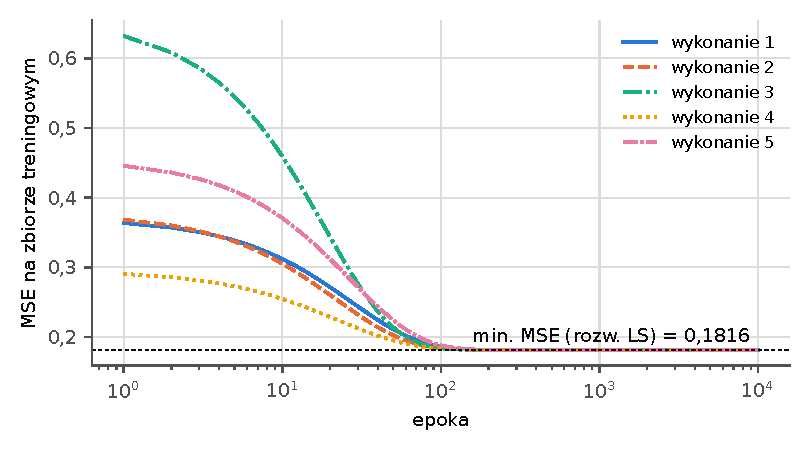
\includegraphics[width=12cm]{mse_N2_M6.pdf}
 \vspace{-0.3cm}
 \caption{Przebieg MSE w~kolejnych epokach dla $N=2$, $M=6$ (oś epok logarytmiczna)}
 \label{fig_n2m6}
\end{figure}

\noindent Mimo różnych punktów startowych wszystkie wykonania zakończyły się
\textbf{identycznymi wagami} -- maksymalna odległość między nimi wynosi
$3{,}8\cdot10^{-15}$, czyli błąd zaokrągleń arytmetyki zmiennoprzecinkowej.
Błąd nie spadł jednak do zera: po ok.~100 epokach ustalił się na poziomie
$\mathrm{MSE}=0{,}1816$, równym minimum osiągalnemu przez rozwiązanie LS
(Rys.~\ref{fig_n2m6}), a~błąd dla najgorszego wzorca to $0{,}689$.
Neuron \textbf{nie został nauczony bezbłędnie} -- nie istnieje wektor wag
spełniający jednocześnie wszystkie 6~równań, więc algorytm znajduje
kompromis minimalizujący sumę kwadratów błędów.

Wagi końcowe różnią się od $X^{+}\mathbf{z}$ o~$3{,}2\cdot10^{-3}$. Tab.~\ref{tab_eta}
pokazuje, że różnica ta jest proporcjonalna do $\eta$ (iloraz w~ostatniej kolumnie
jest stały), a~nadwyżka MSE ponad minimum -- do $\eta^2$. Wynika to z~wariantu
\textit{on-line}: gdy układ jest sprzeczny, każdy wzorzec ,,ciągnie'' wagi
w~stronę własnego rozwiązania, więc przy stałym $\eta$ wagi kończą epokę
w~punkcie przesuniętym względem minimum LS. Dla $\eta\to0$ wynik dąży do rozwiązania LS.

\begin{table}[h!]
 \caption{Wpływ $\eta$ na wynik dla $N=2$, $M=6$ ($K=100\,000$)}
 \centering
 \vspace{0.2cm}
 \begin{tabular}{c c c c}
  \hline\hline\\[-0.4cm]
  $\boldsymbol{\eta}$ & $\|\mathbf{w}-X^{+}\mathbf{z}\|$ & $\mathrm{MSE}-\mathrm{MSE}_{LS}$ & $\|\mathbf{w}-X^{+}\mathbf{z}\|/\eta$\\[0.1cm]
  \hline
  0,1 & $3{,}31\cdot 10^{-2}$ & $3{,}36\cdot 10^{-4}$ & 0,331 \\
  0,03 & $9{,}73\cdot 10^{-3}$ & $2{,}91\cdot 10^{-5}$ & 0,324 \\
  0,01 & $3{,}23\cdot 10^{-3}$ & $3{,}19\cdot 10^{-6}$ & 0,323 \\
  0,003 & $9{,}66\cdot 10^{-4}$ & $2{,}86\cdot 10^{-7}$ & 0,322 \\
  0,001 & $3{,}22\cdot 10^{-4}$ & $3{,}18\cdot 10^{-8}$ & 0,322 \\
  \hline
 \end{tabular}
 \label{tab_eta}
\end{table}

%%%%%%%%%%%%%%%%%%%%%%%%%%%%%%%%%%%%%%%%%%%%%%%%%%%%%%%%%%%%%%%%%%%%%%%%%%%%%%%%%%%%%%%%%%%%%%%%%%%%%%%%%%%%%%%%%
% PODROZDZIAŁ PT. EKSPERYMENT NR 2
%%%%%%%%%%%%%%%%%%%%%%%%%%%%%%%%%%%%%%%%%%%%%%%%%%%%%%%%%%%%%%%%%%%%%%%%%%%%%%%%%%%%%%%%%%%%%%%%%%%%%%%%%%%%%%%%%

\newpage
\subsection{Eksperyment nr 2 -- liczba wag równa liczbie wzorców ($N=M=4$)}

\subsubsection{Założenia}

Układ 4~równań z~4~niewiadomymi. Macierz $X$ jest nieosobliwa (rząd~4),
jej wartości osobliwe to $1{,}672$; $1{,}169$; $1{,}047$; $0{,}246$,
a~współczynnik uwarunkowania $\mathrm{cond}(X)=6{,}79$. Układ ma więc dokładnie
jedno rozwiązanie $X^{-1}\mathbf{z}$.

\subsubsection{Przebieg}

Jak w~eksperymencie nr~1: 5~wykonań z~różnych wag początkowych, porównanie wag
końcowych między sobą i~z~$X^{-1}\mathbf{z}$. Ze względu na wolniejszą zbieżność
dodatkowo powtórzono trening dla $K = 30\,000$ epok.

\subsubsection{Rezultat}

\begin{table}[h!]
 \caption{Wagi końcowe dla $N=M=4$ ($K=10\,000$)}
 \centering
 \vspace{0.2cm}
 \begin{tabular}{c c c c c c c}
  \hline\hline\\[-0.4cm]
  \textbf{Wyk.} & $w_1$ & $w_2$ & $w_3$ & $w_4$ & \textbf{MSE} & $\|\mathbf{w}-X^{-1}\mathbf{z}\|$\\[0.1cm]
  \hline
  \textbf{1} & 1,8519 & 0,7432 & $-$2,1381 & 1,8193 & $8{,}1\cdot 10^{-7}$ & $7{,}3\cdot 10^{-3}$ \\
  \textbf{2} & 1,8519 & 0,7432 & $-$2,1381 & 1,8193 & $8{,}1\cdot 10^{-7}$ & $7{,}3\cdot 10^{-3}$ \\
  \textbf{3} & 1,8506 & 0,7424 & $-$2,1368 & 1,8181 & $1{,}4\cdot 10^{-6}$ & $9{,}7\cdot 10^{-3}$ \\
  \textbf{4} & 1,8521 & 0,7433 & $-$2,1382 & 1,8195 & $7{,}4\cdot 10^{-7}$ & $7{,}0\cdot 10^{-3}$ \\
  \textbf{5} & 1,8522 & 0,7434 & $-$2,1384 & 1,8196 & $6{,}9\cdot 10^{-7}$ & $6{,}8\cdot 10^{-3}$ \\
  \hline
  $X^{-1}z$ & 1,8559 & 0,7459 & $-$2,1420 & 1,8232 & 0 & 0 \\[0.1cm]
  \hline
 \end{tabular}
 \label{tab_n4m4}
\end{table}

\begin{figure}[h!]
 \centering
 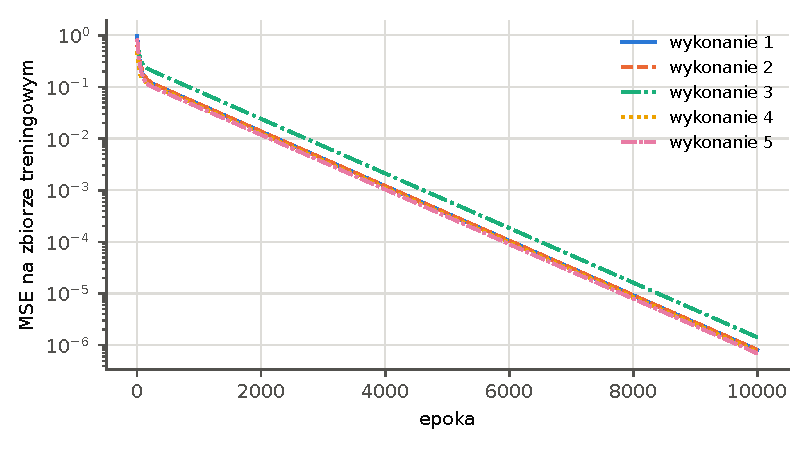
\includegraphics[width=12cm]{mse_N4_M4.pdf}
 \vspace{-0.3cm}
 \caption{Przebieg MSE w~kolejnych epokach dla $N=M=4$ (oś błędu logarytmiczna)}
 \label{fig_n4m4}
\end{figure}

\noindent Na Rys.~\ref{fig_n4m4} błąd maleje wykładniczo (prosta w~skali
logarytmicznej) i~w~granicy dąży do zera -- \textbf{trening bezbłędny jest możliwy}.
Po $10\,000$ epokach MSE wynosi $7\cdot10^{-7}$--$1{,}4\cdot10^{-6}$, a~maksymalny
błąd dla pojedynczego wzorca nie przekracza $1{,}6\cdot10^{-3}$. Wagi końcowe z~różnych
wykonań pokrywają się do trzeciego miejsca po przecinku (maksymalna odległość
$2{,}9\cdot10^{-3}$, Tab.~\ref{tab_n4m4}); pozostała różnica wynika wyłącznie
z~niezakończonej zbieżności. Po $30\,000$ epokach odległość każdego wykonania
od $X^{-1}\mathbf{z}$ spadła do $5{,}0\cdot10^{-8}$, więc wszystkie wykonania
zbiegają do \textbf{tego samego, jedynego rozwiązania}.

Zbieżność jest tu wyraźnie wolniejsza niż w~eksperymencie nr~1. Najwolniej
korygowana jest składowa wag w~kierunku związanym z~najmniejszą wartością osobliwą
$\sigma_{\min}=0{,}246$ -- im gorzej uwarunkowany układ, tym więcej epok potrzeba.

%%%%%%%%%%%%%%%%%%%%%%%%%%%%%%%%%%%%%%%%%%%%%%%%%%%%%%%%%%%%%%%%%%%%%%%%%%%%%%%%%%%%%%%%%%%%%%%%%%%%%%%%%%%%%%%%%
% PODROZDZIAŁ PT. EKSPERYMENT NR 3
%%%%%%%%%%%%%%%%%%%%%%%%%%%%%%%%%%%%%%%%%%%%%%%%%%%%%%%%%%%%%%%%%%%%%%%%%%%%%%%%%%%%%%%%%%%%%%%%%%%%%%%%%%%%%%%%%

\newpage
\subsection{Eksperyment nr 3 -- więcej wag niż wzorców ($N=6$, $M=3$)}

\subsubsection{Założenia}

Układ 3~równań z~6~niewiadomymi. Rząd $X$ wynosi~3, więc $\dim\ker X = N-M = 3$:
rozwiązań jest nieskończenie wiele i~tworzą trójwymiarową podprzestrzeń afiniczną
w~$\mathbb{R}^6$.

\subsubsection{Przebieg}

5~wykonań z~różnych wag początkowych. Poza porównaniem wag końcowych między sobą
i~z~rozwiązaniem o~minimalnej normie $X^{+}\mathbf{z}$ sprawdzono, czy wagi końcowe
są zgodne z~przewidywaniem~(\ref{eq_pred}), tzn.~obliczono $\|\mathbf{w}-\hat{\mathbf{w}}\|$.

\subsubsection{Rezultat}

\begin{table}[h!]
 \caption{Wagi końcowe dla $N=6$, $M=3$}
 \centering
 \vspace{0.2cm}
 \begin{tabular}{c c c c c c c}
  \hline\hline\\[-0.4cm]
  \textbf{Wyk.} & $w_1$ & $w_2$ & $w_3$ & $w_4$ & $w_5$ & $w_6$\\[0.1cm]
  \hline
  \textbf{1} & 1,0447 & 0,0579 & 0,6460 & $-$0,7345 & 0,3556 & 0,2157 \\
  \textbf{2} & 0,9011 & 0,1433 & 0,3802 & $-$0,2842 & $-$0,1093 & $-$0,0737 \\
  \textbf{3} & 0,0905 & 0,7800 & 0,7457 & $-$0,5782 & $-$0,1847 & 0,2570 \\
  \textbf{4} & 0,9501 & 0,2997 & 0,1050 & 0,5125 & $-$0,3832 & $-$0,4387 \\
  \textbf{5} & 0,6270 & 0,0794 & 0,3630 & $-$0,6584 & $-$0,4106 & $-$0,0129 \\
  \hline
  $X^{+}z$ & 0,5330 & 0,3997 & 0,3637 & $-$0,1725 & $-$0,3982 & $-$0,1093 \\[0.1cm]
  \hline
 \end{tabular}
 \label{tab_n6m3_w}
\end{table}

\begin{table}[h!]
 \caption{Błędy i~odległości wag końcowych dla $N=6$, $M=3$}
 \centering
 \vspace{0.2cm}
 \begin{tabular}{c c c c c c}
  \hline\hline\\[-0.4cm]
  \textbf{Wyk.} & \textbf{MSE} & $\max|z-y|$ & $\|\mathbf{w}-X^{+}\mathbf{z}\|$ & $\|\mathbf{w}-\hat{\mathbf{w}}\|$ & $\|\mathbf{w}\|$\\[0.1cm]
  \hline
  \textbf{1} & $7{,}0\cdot 10^{-30}$ & $3{,}3\cdot 10^{-15}$ & 1,2034 & $1{,}5\cdot 10^{-14}$ & 1,4915 \\
  \textbf{2} & $1{,}3\cdot 10^{-30}$ & $1{,}7\cdot 10^{-15}$ & 0,5466 & $8{,}7\cdot 10^{-15}$ & 1,0370 \\
  \textbf{3} & $4{,}5\cdot 10^{-30}$ & $3{,}2\cdot 10^{-15}$ & 0,9114 & $1{,}3\cdot 10^{-14}$ & 1,2678 \\
  \textbf{4} & $5{,}7\cdot 10^{-30}$ & $3{,}1\cdot 10^{-15}$ & 0,9104 & $7{,}7\cdot 10^{-15}$ & 1,2670 \\
  \textbf{5} & $6{,}2\cdot 10^{-30}$ & $3{,}3\cdot 10^{-15}$ & 0,5975 & $8{,}1\cdot 10^{-15}$ & 1,0646 \\
  \hline
  $X^{+}z$ & 0 & 0 & 0 & -- & 0,8812 \\[0.1cm]
  \hline
 \end{tabular}
 \label{tab_n6m3_e}
\end{table}

\begin{figure}[h!]
 \centering
 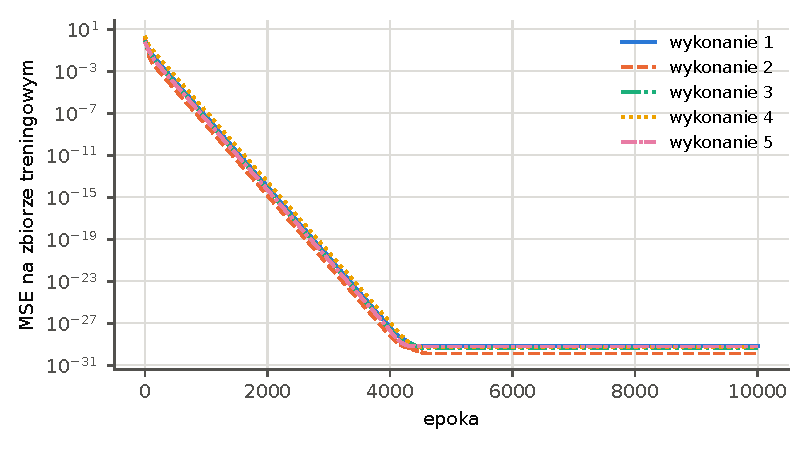
\includegraphics[width=12cm]{mse_N6_M3.pdf}
 \vspace{-0.3cm}
 \caption{Przebieg MSE w~kolejnych epokach dla $N=6$, $M=3$ (oś błędu logarytmiczna)}
 \label{fig_n6m3}
\end{figure}

\noindent W~każdym wykonaniu \textbf{trening był skuteczny}: MSE spadł do
poziomu $10^{-30}$, czyli do granicy precyzji liczb typu \texttt{float64}
(Rys.~\ref{fig_n6m3}, po ok.~4\,500 epokach), a~błąd dla żadnego wzorca nie
przekracza $3{,}4\cdot10^{-15}$. Jednocześnie \textbf{wagi końcowe są w~każdym
wykonaniu inne} (Tab.~\ref{tab_n6m3_w}) -- maksymalna odległość między nimi wynosi
$1{,}76$. Każdy z~tych wektorów jest równie dobrym rozwiązaniem układu.

Tab.~\ref{tab_n6m3_e} potwierdza przewidywanie~(\ref{eq_pred}): wagi końcowe
różnią się od $\hat{\mathbf{w}}$ jedynie o~$10^{-14}$, a~więc są w~pełni wyznaczone
przez wagi początkowe. Trening ,,poprawia'' tylko składową wag w~przestrzeni
rozpiętej przez wzorce, a~składowa z~$\ker X$ pozostaje taka, jaką wylosowano.
Żadne wykonanie nie trafiło w~rozwiązanie o~minimalnej normie
($\|X^{+}\mathbf{z}\|=0{,}881$, podczas gdy $\|\mathbf{w}\|\in[1{,}037;\,1{,}492]$);
osiągnęłoby je tylko wykonanie startujące z~$\mathbf{w}_0=\mathbf{0}$.

%%%%%%%%%%%%%%%%%%%%%%%%%%%%%%%%%%%%%%%%%%%%%%%%%%%%%%%%%%%%%%%%%%%%%%%%%%%%%%%%%%%%%%%%%%%%%%%%%%%%%%%%%%%%%%%%%
% PODROZDZIAŁ PT. EKSPERYMENT NR 4
%%%%%%%%%%%%%%%%%%%%%%%%%%%%%%%%%%%%%%%%%%%%%%%%%%%%%%%%%%%%%%%%%%%%%%%%%%%%%%%%%%%%%%%%%%%%%%%%%%%%%%%%%%%%%%%%%

\subsection{Eksperyment nr 4 -- interpretacja geometryczna}

\subsubsection{Założenia}

Aby zobrazować wyniki eksperymentów 1--3, użyto neuronu o~$N=2$ wagach,
dla którego przestrzeń wag jest płaszczyzną. Każde równanie
$\mathbf{w}^{T}\mathbf{x}^{\mu}=z^{\mu}$ jest w~niej prostą. Wylosowano 3~wzorce
(ziarno 18) i~trenowano neuron kolejno na pierwszym wzorcu ($M=1$), dwóch ($M=2$)
i~trzech ($M=3$), za każdym razem z~tych samych 5~punktów startowych.
Dla czytelności trajektorii przyjęto $\eta=0{,}1$ i~$K=300$.

\subsubsection{Przebieg}

Po każdej poprawce wag zapisywano położenie wektora $\mathbf{w}$ i~rysowano
trajektorie na tle poziomic funkcji MSE.

\subsubsection{Rezultat}

\begin{figure}[h!]
 \centering
 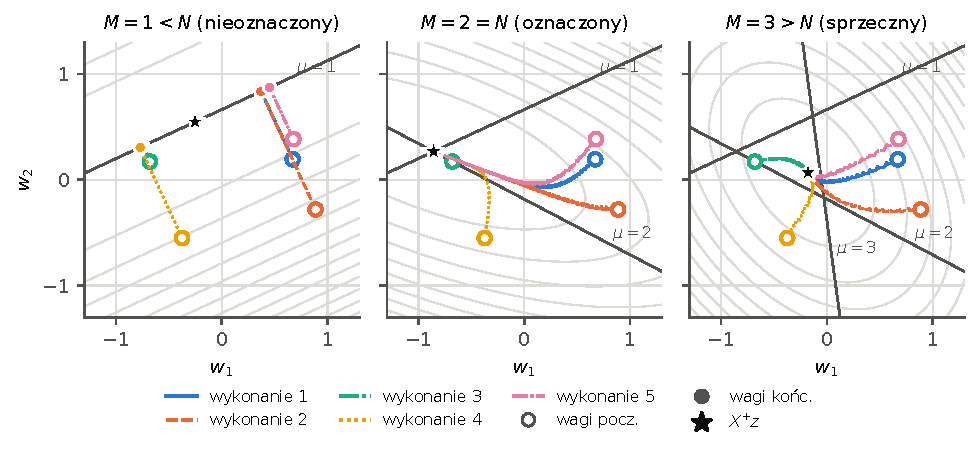
\includegraphics[width=\linewidth]{geometria_2d.pdf}
 \vspace{-0.6cm}
 \caption{Trajektorie wag w~płaszczyźnie $(w_1, w_2)$; szare proste -- równania
 $\mathbf{w}^{T}\mathbf{x}^{\mu}=z^{\mu}$, szare krzywe -- poziomice MSE}
 \label{fig_geom}
\end{figure}

\noindent Rys.~\ref{fig_geom} pokazuje wszystkie trzy przypadki na raz:
\begin{itemize}
 \item $M=1<N$ -- rozwiązania wypełniają całą prostą. Każda trajektoria biegnie
       prostopadle do niej, więc wagi końcowe są rzutem ortogonalnym wag początkowych
       na prostą -- różne dla każdego wykonania (odpowiednik eksperymentu nr~3).
 \item $M=2=N$ -- dwie proste przecinają się w~jednym punkcie i~wszystkie trajektorie
       do niego zbiegają (odpowiednik eksperymentu nr~2).
 \item $M=3>N$ -- trzy proste nie mają wspólnego punktu (układ sprzeczny), więc
       zerowy błąd jest nieosiągalny. Wszystkie trajektorie kończą się w~tym samym
       punkcie wewnątrz trójkąta utworzonego przez proste, w~pobliżu rozwiązania LS;
       widoczne drobne zygzaki to efekt poprawek \textit{on-line} od kolejnych
       wzorców (odpowiednik eksperymentu nr~1).
\end{itemize}

\newpage

\section{Wnioski}

\begin{table}[h!]
 \caption{Zestawienie wyników eksperymentów 1--3}
 \centering
 \vspace{0.2cm}
 \begin{tabular}{c c c c}
  \hline\hline\\[-0.4cm]
   & $\boldsymbol{N<M}$ & $\boldsymbol{N=M}$ & $\boldsymbol{N>M}$\\[0.1cm]
  \hline
  \textbf{Układ równań} & sprzeczny & oznaczony & nieoznaczony \\
  \textbf{Końcowe MSE} & $0{,}1816$ ($=\mathrm{MSE}_{LS}$) & $\to 0$ & $\approx 10^{-30}$ \\
  \textbf{Wagi końcowe} & identyczne & identyczne & różne \\
  \textbf{Zależność od $\mathbf{w}_0$} & brak & brak & wzór~(\ref{eq_pred}) \\
  \textbf{Skuteczny trening} & nie & tak & tak \\[0.1cm]
  \hline
 \end{tabular}
 \label{tab_zestawienie}
\end{table}

\begin{enumerate}
 \item Trening neuronu liniowego regułą delta jest iteracyjnym rozwiązywaniem
       układu $X\mathbf{w}=\mathbf{z}$, a~wszystkie obserwacje (Tab.~\ref{tab_zestawienie})
       wynikają z~tego, ile rozwiązań ma ten układ.
 \item Dla $N<M$ układ jest sprzeczny, więc \textbf{bezbłędny trening nie jest możliwy}.
       Algorytm znajduje jedno, niezależne od wag początkowych rozwiązanie
       kompromisowe, bliskie rozwiązaniu najmniejszych kwadratów. W~wariancie
       \textit{on-line} ze stałym $\eta$ jest ono przesunięte względem LS
       o~wartość proporcjonalną do $\eta$.
 \item Dla $N=M$ (przy $\det X\neq0$) układ ma jedno rozwiązanie: trening jest skuteczny,
       a~wagi końcowe nie zależą od punktu startowego. Liczba potrzebnych epok rośnie
       wraz z~pogarszaniem się uwarunkowania macierzy wzorców.
 \item Dla $N>M$ trening jest zawsze skuteczny, ale wagi końcowe nie są jednoznaczne:
       reguła delta zmienia wagi tylko w~przestrzeni rozpiętej przez wzorce, a~składowa
       wag początkowych z~$\ker X$ przechodzi bez zmian do wyniku. Wagi końcowe
       są dokładnie przewidywane wzorem~(\ref{eq_pred}).
 \item O~niejednoznaczności decyduje właściwie $\dim\ker X = N - \mathrm{rank}\,X$,
       a~nie samo porównanie $N$ i~$M$: przy liniowo zależnych wzorcach podobny efekt
       wystąpiłby także dla $N\le M$.
 \item Praktyczny wniosek: neuron o~większej liczbie wag niż wzorców dopasowuje
       zbiór treningowy bez błędu, ale jego wagi są w~dużej części losowe, więc
       zerowy błąd treningowy nie świadczy o~poprawnym modelu. Potrzeba wtedy więcej
       danych lub dodatkowego kryterium wyboru rozwiązania (np.~minimalnej normy).
\end{enumerate}

%%%%%%%%%%%%%%%%%%%%%%%%%%%%%%%%%%%%%%%%%%%%%%%%%%%%%%%%%%%%%%%%%%%%%%%%%%%%%%%%%%%%%%%%%%%%%%%%%%%%%%%%%%%%%%%%%
% PODROZDZIAŁ PT. ZALACZNIKI
%%%%%%%%%%%%%%%%%%%%%%%%%%%%%%%%%%%%%%%%%%%%%%%%%%%%%%%%%%%%%%%%%%%%%%%%%%%%%%%%%%%%%%%%%%%%%%%%%%%%%%%%%%%%%%%%%

\section{Załączniki}

Implementacja reguły delta (fragment pliku \texttt{neuron\_liniowy.py}).
Pełny kod eksperymentów i~wykresów znajduje się w~plikach
\texttt{neuron\_liniowy.py} oraz \texttt{wykresy.py}.

\begin{lstlisting}[language=Python]
def delta_training(X, Z, eta=0.01, K=100, w_range=(-1, 1), rng=None):
    """Regula delta on-line: po kazdym wzorcu w <- w + eta*(z - y)*x."""
    rng = rng or np.random.default_rng()
    M, N = X.shape
    w0 = rng.uniform(w_range[0], w_range[1], N)
    w = w0.copy()
    mse = np.empty(K)
    for k in range(K):
        for mu in range(M):
            y = w @ X[mu]
            e = Z[mu] - y
            w = w + eta * e * X[mu]
        mse[k] = np.mean((Z - X @ w) ** 2)  # blad na calym zbiorze
    return w0, w, mse
\end{lstlisting}


%%%%%%%%%%%%%%%%%%%%%%%%%%%%%%%%%%%%%%%%%%%%%%%%%%%%%%%%%%%%%%%%%%%%%%%%%%%%%%%%%%%%%%%%%%%%%%%%%%%%%%%%%%%%%%%%%
% BIBLIOGRAFIA
%%%%%%%%%%%%%%%%%%%%%%%%%%%%%%%%%%%%%%%%%%%%%%%%%%%%%%%%%%%%%%%%%%%%%%%%%%%%%%%%%%%%%%%%%%%%%%%%%%%%%%%%%%%%%%%%%

\renewcommand\refname{Bibliografia}
\bibliographystyle{plain}
\bibliography{bibliografia}

\end{document}
